\documentclass[a4paper, 12pt]{examen}

\begin{document}

%\modulo{Prog. multim. y de dispositivos moviles}
%\modulo{Planif. y adm. de redes}
%\modulo{Prog. de servicios y procesos}
\modulo{Lenguajes de marcas}


\pregunta{ Elabora un fichero HTML que consiga exactamente
lo que se muestra en la figura \ref{figura2}. En este ejercicio se debe escribir todo el HTML, incluyendo cabecera,
cuerpo y elementos relevante para la estructura.}{  3.5 }
\begin{figure}[h]
    \caption{Resultado esperable en el ejercicio 1}
    \label{figura2}
    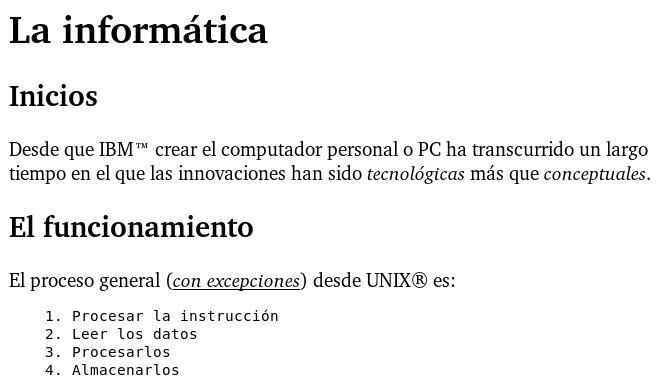
\includegraphics[width=\linewidth]{ej2.png}
\end{figure}
\break

\pregunta{ Elabora un fichero HTML que consiga exactamente
lo que se muestra en la figura \ref{figura2}. En este ejercicio solo hace falta escribir el HTML relevante, es decir, empezar por escribir la etiqueta {\tt table}}{  3.5 }
\begin{figure}[h]
    \caption{Resultado esperable en el ejercicio 2}
    \label{figura2}
    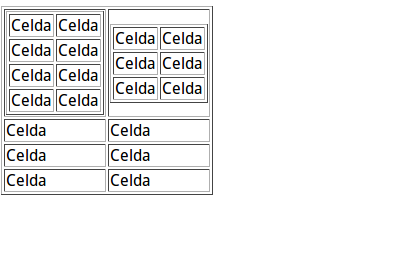
\includegraphics[scale=0.7]{foto_07.png}
\end{figure}
\break



\pregunta{ Elabora un fichero HTML que consiga exactamente
lo que se muestra en la figura \ref{figuraformulario}. En este ejercicio solo hace falta escribir el HTML relevante,
en este caso solo a partir de la etiqueta {\tt form} }{  3.5 }
Ten en cuenta que:

\begin{itemize}





    \item{Hay los siguientes cuadros de texto:cuadro de texto con el texto ``Instituto'' y el name instituto, cuadro de texto con el texto ``Estudios elegidos'' y el name estudios, cuadro de texto con el texto ``Nombre'' y el name nombre, cuadro de texto con el texto ``Apellidos'' y el name apellidos, cuadro de texto con el texto ``Email'' y el name email}

    \item{Hay un control para elegir el color.}

    \item{Hay un textarea que mide 5 filas y 47 columnas que lleva dentro el texto ``Utilice este recuadro por favor''}

    \item{Contiene los siguientes radiobuttons:radio con el name ``red'' , value ``red2g'' y el texto ``2G'', radio con el name ``red'' , value ``red3g'' y el texto ``3G'', radio con el name ``red'' , value ``red4g'' y el texto ``4G''.}

    \item{Hay un control para indicar la fecha.}

    \item{Hay un control para elegir ficheros.}

    \item{Hay una lista desplegable con el name ``conector'' y con las siguientes opciones: opción ``USB'' con el value usb, opción ``Paralelo'' con el value paralelo, opción ``PS2'' con el value ps2.}

    \item{Contiene los siguientes radiobuttons:radio con el name ``sistema'' , value ``sistemawindows'' y el texto ``Windows'', radio con el name ``sistema'' , value ``sistemamac'' y el texto ``Mac'', radio con el name ``sistema'' , value ``sistemalinux'' y el texto ``Linux''.}


\end{itemize}


\begin{figure}[h]
    \caption{Resultado esperable en el ejercicio del formulario.}
    \label{figuraformulario}
    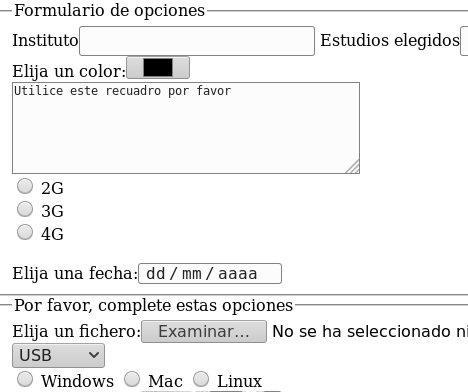
\includegraphics[scale=0.7]{foto_formulario_12.png}
\end{figure}


\end{document}
